\documentclass[UTF8,linespread=1.236]{ctexart}
\usepackage{subfig}
\usepackage{listings}
\usepackage{amsmath}
\usepackage{amssymb}
\usepackage{booktabs}
\usepackage{float}
\usepackage[Q=yes]{examplep}
\usepackage[a4paper,centering,top=3cm,left=2.6cm]{geometry}
\usepackage{pgf}
\usepackage{tikz}
\usetikzlibrary{arrows,automata,positioning}

\pagestyle{plain}
\ctexset {
    section = {
        name = {},
        number = {},
        aftername = {},
    },
    subsection = {
        name = {,、},
        number = \chinese{subsection},
        aftername = {},
    },
    subsubsection = {
        name = {},
        number = \arabic{subsubsection},
    }
}
\newcommand\myref[1]{(\ref{#1})}
\newcommand\cu[1]{\boldsymbol{#1}}
\newcommand\vecE{\cu{E}}
\newcommand\vecH{\cu{H}}
\newcommand\pypx[2]{{{\partial {#1}} \over {\partial {#2}}}}
\newcommand\pie{{}^\prime}
\newcommand\nextsign{{}^\ast}
\begin{document}

\title{《电磁场与波B》课程设计}
\author{电子科学与工程学院\ \ 傅宣登 (2016030102010)}

\maketitle
%\thispagestyle{empty}

\section{关于均匀平面波与圆极化波的性质能否同时满足的探讨}

\subsection{均匀平面波}

\subsubsection{一般波动方程}

对于电容率为 $\varepsilon$,磁导率为 $\mu$,电导率为 $\sigma$
的无源均匀媒质,
麦克斯韦方程是
\begin{equation}%\label{eq81}
    \nabla \times \cu{E} = - \pypx{\cu{B}}{t}
\end{equation}
\begin{equation}
    %\label{eq82}
    \nabla \times \cu{H} = \cu{J} + \pypx{\cu{D}}{t}
\end{equation}
\begin{equation}
    %\label{eq83}
    \nabla \cdot \cu{B} = 0
\end{equation}
\begin{equation}
    %\label{eq84}
    \nabla \cdot \cu{D} = \rho
\end{equation}
其中 $\cu{J} = \sigma\cu{E}$,$\cu{B} = \mu\cu{H}$,
$\cu{D} = \varepsilon\cu{E}$,
$\rho = 0$. 于是有
\begin{equation}
    \label{eq81}
    \nabla \times \cu{E} = -\mu \pypx{\cu{H}}{t}
\end{equation}
\begin{equation}
    \label{eq82}
    \nabla \times \cu{H} = \sigma\cu{E} + \varepsilon\pypx{\cu{E}}{t}
\end{equation}
\begin{equation}
    \label{eq83}
    \nabla \cdot \cu{H} = 0
\end{equation}
\begin{equation}
    \label{eq84}
    \nabla \cdot \cu{E} = 0
\end{equation}

上述方程只与两个变量($\vecE$ 和 $\vecH$)有关,
进一步可得出一个变量的方程.

对式 \myref{eq81} 两边取旋度得
\begin{equation}\label{eq85}
    \nabla \times \nabla \times \vecE
    =
    - \mu \nabla \times \left( \pypx{\vecH}{t} \right)
\end{equation}
由矢量恒等式
\begin{equation}
    \nabla \times \nabla \times \vecE
    =
    \nabla(\nabla \cdot \vecE)
    -
    \nabla^2\vecE
\end{equation}
以及 $\nabla \cdot \vecE = 0$ 得
\begin{equation}
    \nabla \times \nabla \times \vecE = - \nabla^2\vecE
\end{equation}
在直角坐标系下
\begin{equation}
    \nabla^2 =
    \nabla^2E_x\cu{a}_x +
    \nabla^2E_y\cu{a}_y +
    \nabla^2E_z\cu{a}_z
\end{equation}
其中拉普拉斯算子为
\begin{equation}
    \nabla^2 = \pypx{^2}{x^2} + \pypx{^2}{y^2} + \pypx{^2}{z^2}
\end{equation}
改变对空间和时间微分的顺序,式\myref{eq85}重写为
\begin{equation*}
    \nabla^2\vecE = \mu \pypx{}{t}\left[ \nabla \times \vecH \right]
\end{equation*}
将式\myref{eq82}带入上式得
\begin{equation}
    \nabla^2\vecE = 
    \mu \sigma \pypx{\vecE}{t} + \mu \varepsilon \pypx{^2\vecE}{t^2}
\end{equation}
同理可得
\begin{equation}
    \nabla^2\vecH = 
    \mu \sigma \pypx{\vecH}{t} + \mu \varepsilon \pypx{^2\vecE}{t^2}
\end{equation}
上述两个方程即是一般波动方程,
支配着无源均匀导电媒质中电磁场的行为.

\subsubsection{无耗介质中的平面波}
令 $\sigma = 0$,得到无耗媒质中的波动方程为
\begin{equation}
    \nabla^2 \vecE - \mu\varepsilon\pypx{^2\vecE}{t^2} = 0
\end{equation}
\begin{equation}
    \nabla^2 \vecH - \mu\varepsilon\pypx{^2\vecH}{t^2} = 0
\end{equation}
这两个方程也称为时变赫姆霍兹方程.
式中没有一阶项,表明电磁场在无耗媒质中传播时是不衰减的.

接下来考虑常量 $\vecE$ 和 $\vecH$ 的分量都在与波的传播方向垂直的平面的波,
这种波即被称为平面波.
假定波沿 $x$ 方向传播,
则 $\vecE$ 和 $\vecH$ 场
均无纵向分量,即
\begin{equation*}
    E_x = 0 \quad H_x = 0
\end{equation*}

\subsubsection{均匀平面波的特点}
在平面波中,均匀平面波是最简单和最易理解的一种波.
均匀的意思是
在任意时刻在所在的平面中场的大小和方向都是不变的.
所以对于沿 $x$ 方向传播的均匀平面波,
$\vecE$ 和 $\vecH$ 都不是 $z$ 和 $y$ 的函数,即
\begin{equation} \label{eqpmb}
\begin{aligned}
    \pypx{\vecE}{z} = 0 \quad \pypx{\vecE}{y} = 0 \\
    \pypx{\vecH}{z} = 0 \quad \pypx{\vecH}{y} = 0
\end{aligned}
\end{equation}
这表明场分量只是 $x$(传播方向) 和 $t$(时间) 的函数,
如
\begin{equation}
    E_y(x,t) = E_{ym}\cos{(\omega t - kx + \phi_y)}
\end{equation}
均匀平面波也可表述为:同相面上,各个点的场强都是相等的.

\subsection{圆极化波}

\subsubsection{极化的概念}
\newcommand\phase[1]{\omega t - kx + \phi_{#1}}
一般情况下,
沿 $x$ 方向传播的均匀平面波的 $E_y$ 和 $E_z$ 都存在,
可以表示为
\begin{equation}
    E_y = E_{ym}\cos{(\phase{y})}
\end{equation}
\begin{equation}
    E_z = E_{zm}\cos{(\phase{z})}
\end{equation}
合成波电场 $\vecE = \cu{e}_yE_y + \cu{e}_zE_z$.
由于 $E_y$ 和 $E_z$ 分量的振幅和相位不一定相同,
因此,
在空间任意给定点上,合成波电场强度矢量 $\vecE$ 的
大小和方向都可能会随时间变化,这种现象就称为电磁波的极化.

根据电场强度矢量的端点随时间变化的轨迹,
可以将极化分为直线极化、圆极化、椭圆极化和随机极化等.

\subsubsection{圆极化}

当电场强度矢量的端点随时间变化的轨迹为圆时,
这样的波就称为圆极化波.

例如,两电场分量为
\begin{equation}
    E_y(x,t) = E_0\cos{(\phase{y})}
\end{equation}
\begin{equation}
    E_z(x,t) = E_0\sin{(\phase{z})}
\end{equation}
在 $x = 0$ 平面中,它们是
\begin{equation}
    E_y(0,t) = E_0\cos{(\omega t + \phi_y)}
\end{equation}
\begin{equation}
    E_z(0,t) = E_0\sin{(\omega t + \phi_z)}
\end{equation}
两式平方后相加即得
\begin{equation}
    E_y^2(0,t) + E_z^2(0,t) = E_0^2
\end{equation}
显然,这是圆的方程.

\subsection{同时满足两种性质的波}

考虑两列振幅相等、
传播方向相同、
偏振方向互相垂直、
相位差 $\pi \over 2$ 的均匀平面波的叠加.

不失一般性,设波的两个分量 $E_z$ 和 $E_y$ 为
\begin{gather}
    E_z(x,t) = \cos{(\omega t + kx)} \\
    E_y(x,t) = \cos{(\omega t + kx + {\pi \over 2})}
\end{gather}
合场强 $\vecE$ 为
\begin{equation}
    \vecE = \cu{e}_zE_z + \cu{e}_yE_y
\end{equation}

\subsubsection{满足平面波的特征}
先来验证这个波是个平面波.

将合场强分别对 $y$ 和 $z$ 求偏微分得
\begin{equation}
    \pypx{\vecE}{y} = 0 \qquad \pypx{\vecE}{z} = 0
\end{equation}

上式满足方程 \myref{eqpmb},所以该波是一个平面波.
在等相面 $\omega t + kx = C$ 上每个点的场强都是一样的.

\subsubsection{是圆极化波}
考虑 $x = 0$ 的平面,场强的两个分量为
\begin{align}
E_z(0,t) &= \cos{\omega t} \\
E_y(0,t) &= \cos{(\omega t + {\pi \over 2})} \notag \\
&= -\sin{\omega t}
\end{align}
显然有
\begin{equation}
    E_z^2(0,t) + E_y^2(0,t) = 1
\end{equation}
这是圆的方程,于是该波是一个圆极化波.

\subsubsection*{}

综上所述,本节考虑的波既是均匀平面波、又是圆极化波,
如图 \ref{fig1} 所示.

\begin{figure}[htbp]
\centering
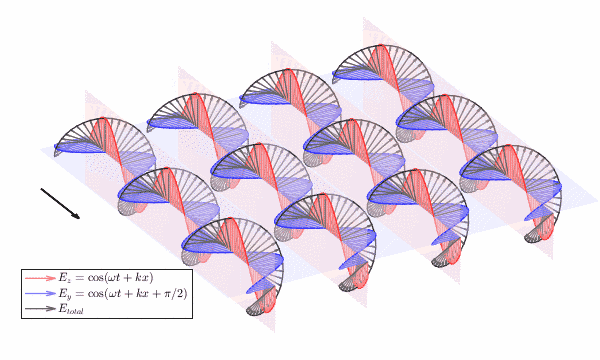
\includegraphics[width=0.6\textwidth]{wave.png}
\caption{该波既是均匀平面波又是圆极化波}\label{fig1}
\end{figure}

\subsection{结论}

通过以上的探讨可以看出,
一个波既是均匀平面波又是
圆极化波是可能的.

均匀平面波是电磁波的空间特性,
圆极化是其时域特性,
两者并无矛盾

\clearpage

\end{document}
